\section{Transfer to a finer mesh}\label{sec:transfer}

\subsection{Zero-shot and few-shot}\label{sec:transfer:zeroshot}

% generated by scripts/make_cmame_material.py from the records; do not edit
\begin{table}[tbp]
\centering
\footnotesize
\setlength{\tabcolsep}{4pt}
\caption{Three-dimensional solids on the finer mesh ($l_c$ = 0.0374), never trained on. Zero-shot rows use the networks trained in-band; few-shot rows train, with labels, on the first 16 or on all of the 64 fine-mesh instances reserved for few-shot training.}
\label{tab:transfer}
\resizebox{\ifdim\width>\textwidth\textwidth\else\width\fi}{!}{%
\begin{tabular}{lccccc}
\toprule
Model & \shortstack{Displacement \\ error} & \shortstack{Relative \\ energy gap} & \shortstack{von Mises \\ error} & \shortstack{Peak stress \\ error} & \shortstack{Critical-region \\ recall} \\
\midrule
Label-free, zero-shot & 0.258 $\pm$ 0.045 & 0.306 $\pm$ 0.220 & 0.305 $\pm$ 0.063 & 0.769 $\pm$ 0.667 & 0.721 $\pm$ 0.006 \\
Supervised (1,024 labels), zero-shot & 0.257 $\pm$ 0.048 & 0.985 $\pm$ 0.267 & 0.537 $\pm$ 0.040 & 2.56 $\pm$ 1.39 & 0.462 $\pm$ 0.028 \\
Graph network (1,024 labels), zero-shot & 0.459 $\pm$ 0.010 & 16.3 $\pm$ 9.6 & 2.40 $\pm$ 0.84 & 11.6 $\pm$ 7.8 & 0.0610 $\pm$ 0.0083 \\
\midrule
Nearest-neighbour field & 0.401 & 4.98 & 1.55 & 3.61 & 0.232 \\
Scaled polynomial & 1.95 & 540 & 18.7 & 134 & 0.102 \\
\midrule
Label-free, then 16 fine-mesh labels & 0.0531 $\pm$ 0.0030 & 0.0702 $\pm$ 0.0112 & 0.166 $\pm$ 0.016 & 0.389 $\pm$ 0.061 & 0.715 $\pm$ 0.004 \\
Supervised from scratch, 16 fine-mesh labels & 0.799 $\pm$ 0.037 & 2.34 $\pm$ 1.25 & 1.07 $\pm$ 0.19 & 2.58 $\pm$ 1.23 & 0.116 $\pm$ 0.014 \\
Label-free, then 64 fine-mesh labels & 0.0298 $\pm$ 0.0020 & 0.0520 $\pm$ 0.0088 & 0.126 $\pm$ 0.018 & 0.272 $\pm$ 0.068 & 0.731 $\pm$ 0.014 \\
Supervised from scratch, 64 fine-mesh labels & 0.193 $\pm$ 0.076 & 13.2 $\pm$ 5.3 & 2.57 $\pm$ 0.47 & 8.94 $\pm$ 4.65 & 0.128 $\pm$ 0.043 \\
\bottomrule
\end{tabular}}

\smallskip
\begin{minipage}{\linewidth}\footnotesize\raggedright
256 fine-mesh evaluation instances (median 36,216 nodes), disjoint from the 64 instances reserved for few-shot training. Mean $\pm$ sample standard deviation over 3 seeds; the naive baselines are deterministic and built from the 1,024 in-band labelled instances.\par
In-band, the label-free network's displacement error is 0.0300; the zero-shot ratio is therefore 8.62.\par
Few-shot training runs 50 epochs at learning rate 1.5 $\times$ 10$^{-3}$ from the trained label-free network of the same seed, or from random initialisation (scratch); the few-shot comparison was pre-registered as reported only.
\end{minipage}
\end{table}


\Cref{tab:transfer} evaluates the networks trained in-band on the 256 fine-mesh evaluation
instances, meshed at $l_c=0.0374$, about half the in-band element size, which no network
had seen. None transferred. The label-free transformer's displacement error rose from
\numAmpInDisp{} in-band to \numFineFreeDisp{}, a factor of \numFineRatio{}; the
pre-registered criterion for transfer allowed \numFineWin{} and the kill condition KP4 was
triggered above \numFineKill{}, so the transfer claim was withdrawn. The supervised transformer
had almost the same displacement error, \numFineLabDisp{}, and the graph network
\numFineMgnDisp{}, worse than the nearest-neighbour field's \numFineKnnDisp{}. The
label-free transformer kept the lowest relative energy gap (\numFineFreeGap{} against
\numFineLabGap{} and \numFineMgnGap{}) and the lowest von Mises error (\numFineFreeVm{}
against \numFineLabVm{} and \numFineMgnVm{}).

Training on a few labelled fine-mesh instances, starting from the trained label-free
network, was
pre-registered as a reported comparison without a criterion. With 64 such instances the
displacement error returned to the in-band level, \numFewSixtyFourDisp{}, and with 16 it
was \numFewSixteenDisp{}, against \numFewSixtyFourScratchDisp{} and
\numFewSixteenScratchDisp{} when the same network was trained from scratch on the same
instances. The relative energy gap, von Mises error and peak stress error did not recover
as far: with 64 instances they remained \numFewFactorMin{} to \numFewFactorMax{} times their
in-band values.

\subsection{On the finer mesh, most of the label-free error is an error of
amplitude}\label{sec:transfer:amplitude}

% generated by scripts/make_cmame_material.py from the records; do not edit
\begin{table}[tbp]
\centering
\footnotesize
\setlength{\tabcolsep}{4pt}
\caption{Post hoc, three-dimensional: errors before and after scaling each prediction by its energy-optimal amplitude $c^*$, in-band and on the finer mesh (zero-shot).}
\label{tab:amplitude}
\resizebox{\ifdim\width>\textwidth\textwidth\else\width\fi}{!}{%
\begin{tabular}{lccccccc}
\toprule
Network & \shortstack{In-band \\ displacement} & \shortstack{In-band \\ with $c^*$} & \shortstack{Fine displacement \\ (zero-shot)} & \shortstack{Fine \\ with $c^*$} & \shortstack{Fine relative \\ energy gap (median)} & \shortstack{Fine \\ with $c^*$} & \shortstack{Median $c^*$ \\ (fine)} \\
\midrule
Transformer & 0.0300 $\pm$ 0.0028 & 0.0142 $\pm$ 0.0032 & 0.258 $\pm$ 0.045 & 0.0832 $\pm$ 0.0158 & 0.0911 $\pm$ 0.0177 & 0.0418 $\pm$ 0.0031 & 1.23 $\pm$ 0.08 \\
Bottleneck, M = 512 & 0.106 $\pm$ 0.051 & 0.0393 $\pm$ 0.0243 & 0.463 $\pm$ 0.082 & 0.124 $\pm$ 0.039 & 0.258 $\pm$ 0.075 & 0.0904 $\pm$ 0.0405 & 1.73 $\pm$ 0.42 \\
Bottleneck, M = 1,024 & 0.0892 $\pm$ 0.0096 & 0.0292 $\pm$ 0.0049 & 0.574 $\pm$ 0.059 & 0.126 $\pm$ 0.037 & 0.263 $\pm$ 0.037 & 0.0717 $\pm$ 0.0326 & 1.77 $\pm$ 0.28 \\
\bottomrule
\end{tabular}}

\smallskip
\begin{minipage}{\linewidth}\footnotesize\raggedright
$c^*$ = $F^\top u / (u^\top K u)$, per load case: the energy-optimal amplitude of the prediction $u$ on the evaluated mesh, from that mesh's stiffness matrix $K$ and load vector $F$ (no labels, no solve). Scaling by $c^*$ never increases the error in the energy norm (it did not in any of the 4,608 instance-seed evaluations measured). In-band median $c^*$: 1.00 (transformer), 1.00 (M = 512), 1.00 (M = 1,024).\par
Seeds per network: 3; seed mean $\pm$ sample SD of the per-seed mean over instances (relative energy gap: per-seed median). In-band: the 256 validation instances; fine: 256 instances at $l_c$ = 0.0374, never trained on. The columns without $c^*$ reproduce the runs' own per-instance arrays: the transformer's exactly, the bottleneck's to a relative 0.011 at most; the bottleneck run's own two evaluations of the same trained networks (in-band) differ by up to 0.003, the transformer run's not at all.\par
Mean fine relative energy gap over instances (a heavy tail), as trained $\rightarrow$ with $c^*$: transformer: 0.306 $\rightarrow$ 0.0670; M = 512: 0.295 $\rightarrow$ 0.106; M = 1,024: 0.590 $\rightarrow$ 0.0984.\par
Measured after the runs; no verdict is revisited.
\end{minipage}
\end{table}


Rescaling each prediction by its energy-optimal amplitude $\cstar$ (\cref{prop:amp}),
which needs no label and no solve, separates errors of amplitude from errors of shape. We
measured it after the runs, on the stored networks (\cref{tab:amplitude}); no verdict was
revisited. On the finer mesh the median $\cstar$ of the label-free transformer was
\numAmpFineCstar{}, against \numAmpInCstar{} in-band: its predictions were too small.
Rescaling lowered its fine-mesh displacement error from \numAmpFineDisp{} to
\numAmpFineDispC{}, by \numAmpFineRedMin{} to \numAmpFineRedMax{} in each seed, and the
median relative energy gap from \numAmpFineGapMedian{} to \numAmpFineGapMedianC{}. In-band
it also helped, from \numAmpInDisp{} to \numAmpInDispC{} in displacement and from
\numAmpInGap{} to \numAmpInGapC{} in mean relative energy gap. Measured as KP4 measures
transfer, with $\cstar$ applied on both meshes, the ratio of fine-mesh to in-band
displacement error fell from \numFineRatio{} to \numAmpRatioBoth{}; with $\cstar$ applied
on the finer mesh only it was \numAmpRatioFineOnly{}. Rescaling removes most of the error
but not the failure to transfer.

% generated by scripts/make_cmame_material.py from the records; do not edit
\begin{table}[tbp]
\centering
\footnotesize
\setlength{\tabcolsep}{4pt}
\caption{Post hoc, three-dimensional: the energy-optimal amplitude $c_b$ of the four load cases of an instance together, on fixed geometries and loads meshed at four mesh sizes $l_c$.}
\label{tab:remesh}
\resizebox{\ifdim\width>\textwidth\textwidth\else\width\fi}{!}{%
\begin{tabular}{lcccc}
\toprule
Network & $l_c$ = 0.0906 & $l_c$ = 0.0742 & $l_c$ = 0.0579 & \shortstack{$l_c$ = 0.0374 \\ (fine)} \\
\midrule
Transformer & 0.98 $\pm$ 0.00 & 1.00 $\pm$ 0.01 & 1.01 $\pm$ 0.00 & 1.27 $\pm$ 0.08 \\
Bottleneck, M = 512 & 0.91 $\pm$ 0.04 & 1.00 $\pm$ 0.02 & 1.14 $\pm$ 0.09 & 1.96 $\pm$ 0.46 \\
Bottleneck, M = 1,024 & 0.94 $\pm$ 0.01 & 1.01 $\pm$ 0.01 & 1.14 $\pm$ 0.02 & 1.99 $\pm$ 0.35 \\
\bottomrule
\end{tabular}}

\smallskip
\begin{minipage}{\linewidth}\footnotesize\raggedright
16 fresh geometries, each meshed at the 4 $l_c$ with identical geometry and loads, so only the mesh changes; every mesh evaluated by every seed. $c_b$: the single energy-optimal amplitude of all four load cases of an instance (label-free, \cref{sec:transfer:amplitude}); median over the geometries, then seed mean $\pm$ sample SD. Training range: $l_c$ = 0.0579--0.0906.\par
The largest nodal load over the four load cases, by which both networks multiply their output, relative to $l_c$ = 0.0906, at $l_c$ = 0.0742 / 0.0579 / 0.0374: 0.705 / 0.430 / 0.186; for comparison ($l_c$ / 0.0906)$^2$: 0.671 / 0.408 / 0.170.\par
Predicted energy norm relative to $l_c$ = 0.0906 (label-free), seed means, $l_c$ = 0.0742 / 0.0579 / 0.0374: transformer: 0.99 / 0.98 / 0.75; M = 512: 0.90 / 0.82 / 0.50; M = 1,024: 0.93 / 0.83 / 0.49.\par
Measured after the runs.
\end{minipage}
\end{table}


Why the amplitude is wrong on the finer mesh is suggested by \cref{tab:remesh}, also
measured after the runs: \numRemeshGeometries{} new geometries, each meshed at four
characteristic lengths with the same loads, so that only the mesh changes. For each mesh
we computed the single energy-optimal amplitude of all four load cases,
$c_b=\sum_jF_j^{\top}u_j/\sum_ju_j^{\top}Ku_j$, the counterpart of \eqref{eq:cstar} for
the sum of their energies. Over the training range the median $c_b$ of the label-free
transformer stayed within \numRemeshInDev{} of one, and at $l_c=0.0374$ it was
\numRemeshFine{}. The largest nodal load $F_{\max}$, by which the output is multiplied
(\cref{sec:methods:networks}), shrinks with the element size, roughly as $l_c^2$ for the
face tractions, whereas the solution does not depend on the mesh; a finer mesh therefore
asks the network for a larger output than any it produced in training. We have not tested
this explanation causally. It agrees with the two-dimensional observation of
\cref{sec:results2d:other}, where the output was not multiplied by $F_{\max}$ and networks
trained on meshes \numCoarsenLow{} and \numCoarsenHigh{} times coarser lost little accuracy
on the original meshes; but the errors of those networks were probably dominated by the
missing load amplitude (\cref{sec:results2d:julyaccuracy}), so the contrast is suggestive
only. A separate pre-registered
study, outside the scope of this paper, tests an output scale that does not depend on the
mesh. \Cref{fig:field-fine} shows a typical fine-mesh prediction before and after the
rescaling: the prediction has the shape of the solution and too small an amplitude.

\begin{figure}[tbp]
\centering
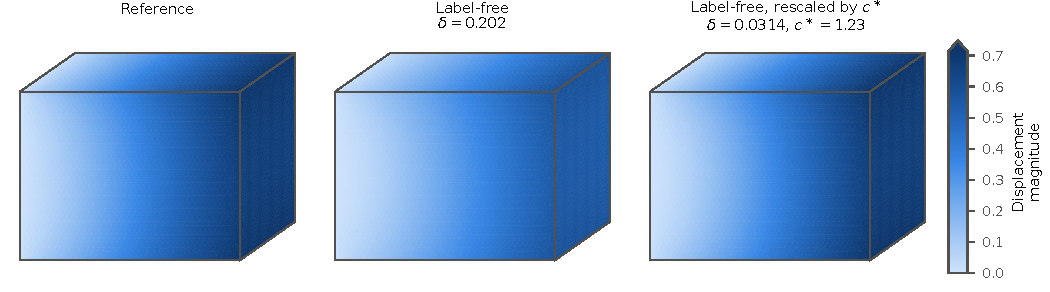
\includegraphics[width=\linewidth]{generated/fig_field_fine.pdf}
\caption{A typical fine-mesh instance, the one with the median displacement error of the
label-free transformer, seed 0, under the \numFigFineLoad{} (selection rules in
\cref{sec:methods:prereg}). Magnitude of the displacement of the reference solution, of the
label-free prediction and of that prediction rescaled by $\cstar$ \eqref{eq:cstar}, on one
colour scale set by the reference and displayed as in \cref{fig:field-worst}; above each
prediction, its relative displacement error $\delta$ on this load case and, for the rescaled
one, $\cstar$.}
\label{fig:field-fine}
\end{figure}
